\documentclass[12pt]{article}
\usepackage[utf8]{inputenc}
\usepackage[spanish]{babel}
\usepackage[letterpaper, top=3cm, bottom=3cm, left=4cm, right=2.5cm]{geometry}
\usepackage{csquotes}
\usepackage{graphicx}
\usepackage{float}
\usepackage{longtable}
\usepackage{caption}
\usepackage{titlesec}
\usepackage{setspace}
\usepackage{fancyhdr}
\usepackage{tocloft}
\usepackage[hidelinks]{hyperref}
\usepackage{pdflscape} % Para páginas horizontales
\usepackage{authblk}
\usepackage[
backend=biber,
style=apa,
sortcites,
url=true
]{biblatex}
\addbibresource{intervencion_empresarial.bib}

%Titulo y autor
\title{Propuesta de implementación de metodología y oficina de proyectos 
\(PO\) 
para la gestión de proyectos de tecnología y control industrial en la empresa S\&G Soluciones de Ingeniería.
}
\author{Mario Javier Serrano Bula}
\date{\today}
% director del trabajo
\newcommand{\mydirector}{Nombre completo del director(a)} 
% universidad
\newcommand{\myuniversity}{Universidad EAN}
% facultad
\newcommand{\myfaculty}{Ingeniería}
% programa
\newcommand{\myprogram}{Maestria en Gerencia de Proyectos}
% ciudad
\newcommand{\mycity}{Bogotá, Colombia}

% ... Titulo del trabajo
\newcommand{\mytitle}{Propuesta de implementación de metodología y oficina de proyectos 
\(PO\) 
para la gestión de proyectos de tecnología y control industrial en la empresa S\&G Soluciones de Ingeniería.
}

\onehalfspacing
\pagestyle{fancy}
\fancyhf{}
\lhead{\footnotesize
  \begin{minipage}[t]{0.8\textwidth}
      \mytitle
  \end{minipage}
}% Encabezado izquierdo
\rhead{\thepage}                           % Encabezado derecho con el número de página
\renewcommand{\cftsecleader}{\cftdotfill{\cftdotsep}}

% Ocultar los títulos de listas
\addto\captionsspanish{
  \renewcommand{\listfigurename}{}
  \renewcommand{\listtablename}{}
}

\newcommand{\chapterbreak}{\clearpage \thispagestyle{fancy}}

\begin{document}
% --------- Portada ---------
% Portada con título y autor
\begin{titlepage}
\makeatletter
\@title\\[3cm]
\@author\\
\makeatother

\vfill
\begin{flushleft}
\myuniversity\\
\myfaculty\\
\myprogram\\
\mycity\\
\today
\end{flushleft}
\end{titlepage}
% --------- Fin Portada ---------

% --------- Página de Presentacion---------
\chapterbreak
\begin{center}
\mytitle\\[2cm]

Trabajo de grado presentado como requisito para optar al título de: Magíster en Gerencia de Proyectos\\[2cm]

Director: \mydirector\\[2cm]
Modalidad: Trabajo Dirigido\\[1.5cm]

\vfill
\myuniversity\\
\myfaculty\\
\myprogram\\
\mycity\\
\today
\end{center}
% --------- Fin Página de Presentacion---------

\chapterbreak
\section*{Nota de Aceptación}
\vspace{4cm}
Firma del jurado\\
Firma del jurado\\
Firma del director del trabajo de grado\\[2cm]
Ciudad, d\'ia/mes/a\~no

\chapterbreak

\section*{Dedicatoria}
\textit{A mis padres por ense\~narme que la exigencia personal tiene sus frutos.}

\chapterbreak
\section*{Agradecimientos}
\paragraph{}
A todas las personas e instituciones que hicieron posible la realizaci\'on de este trabajo.

\chapterbreak
\section*{Resumen}
Incluya las ideas principales de su trabajo de grado: tem\'atica, antecedentes, objetivo, metodolog\'ia, resultados y conclusiones.\\
\textbf{Palabras clave:} hasta 7 palabras

\chapterbreak
\section*{Abstract}
Include topic, background, purpose, methodology, results, and conclusions.\\
\textbf{Keywords:} up to 7 words

% Tabla de contenidos
\chapterbreak
\tableofcontents
\newpage

% Listas de figuras y tablas
\listoffigures
\listoftables

\chapterbreak
\section{Introducción}
\subsection*{Tema de la intervenci\'on empresarial}
\subsection*{Planteamiento del problema}
\subsection*{Pregunta de investigaci\'on}
\subsection*{Estructura del documento}

\chapterbreak
\section{Objetivos}
\begin{flushleft}
A medida que las organizaciones incursionan en nuevos mercados, los desafíos asociados a la gestión efectiva de sus proyectos aumentan significativamente. En este contexto, muchas oportunidades pueden derivar en resultados no satisfactorios, debido a la carencia de un enfoque disciplinado y sistemático en la gestión de proyectos. La gestión de proyectos permite anticipar riesgos, mitigar errores y mejorar la toma de decisiones a lo largo del ciclo de vida.
En relación con lo anterior se establecen los siguientes objetivos que guiarán el desarrollo de esta propuesta:

\subsection*{Objetivo general}
Proponer una metodología de gestión de proyectos y una propuesta de implementación para Oficina de Proyectos (OP), para la empresa S\&G Soluciones de Ingeniería, que facilite la evaluación, formulación y planeación, para la ejecución de sus proyectos de ingeniería y tecnología.
\subsection*{Objetivos específicos}
\begin{itemize}
    \item Diagnosticar la situación actual de la gestión de proyectos en S\&G Soluciones de Ingeniería, e identificar su madurez para la gestión de proyectos.
    \item Diseñar una metodología de gestión de proyectos personalizada para S\&G Soluciones de Ingeniería, basada en las mejores prácticas y marcos reconocidos.
    \item Proponer un plan de implementación gradual para la metodología y Oficina de Proyectos (OP) en S\&G Soluciones de Ingeniería, que actúe como un centro de estandarización, soporte y mejora continua para la gestión de proyectos dentro de la organización.
\end{itemize}
\end{flushleft}

\chapterbreak
\section{Justificaci\'on}
Desarrollar argumentos que sustenten la relevancia, utilidad y viabilidad del proyecto \parencite{hawking2010}.

\chapterbreak

\section{Marco Institucional}
Descripci\'on de la organizaci\'on, su misi\'on, visi\'on, estructura, productos/servicios, sector econ\'omico, etc.

\chapterbreak

\section{Marco de Referencia}
\subsection*{Antecedentes y teor\'ias relevantes}
\subsection*{Figuras}
\begin{figure}[H]
\centering
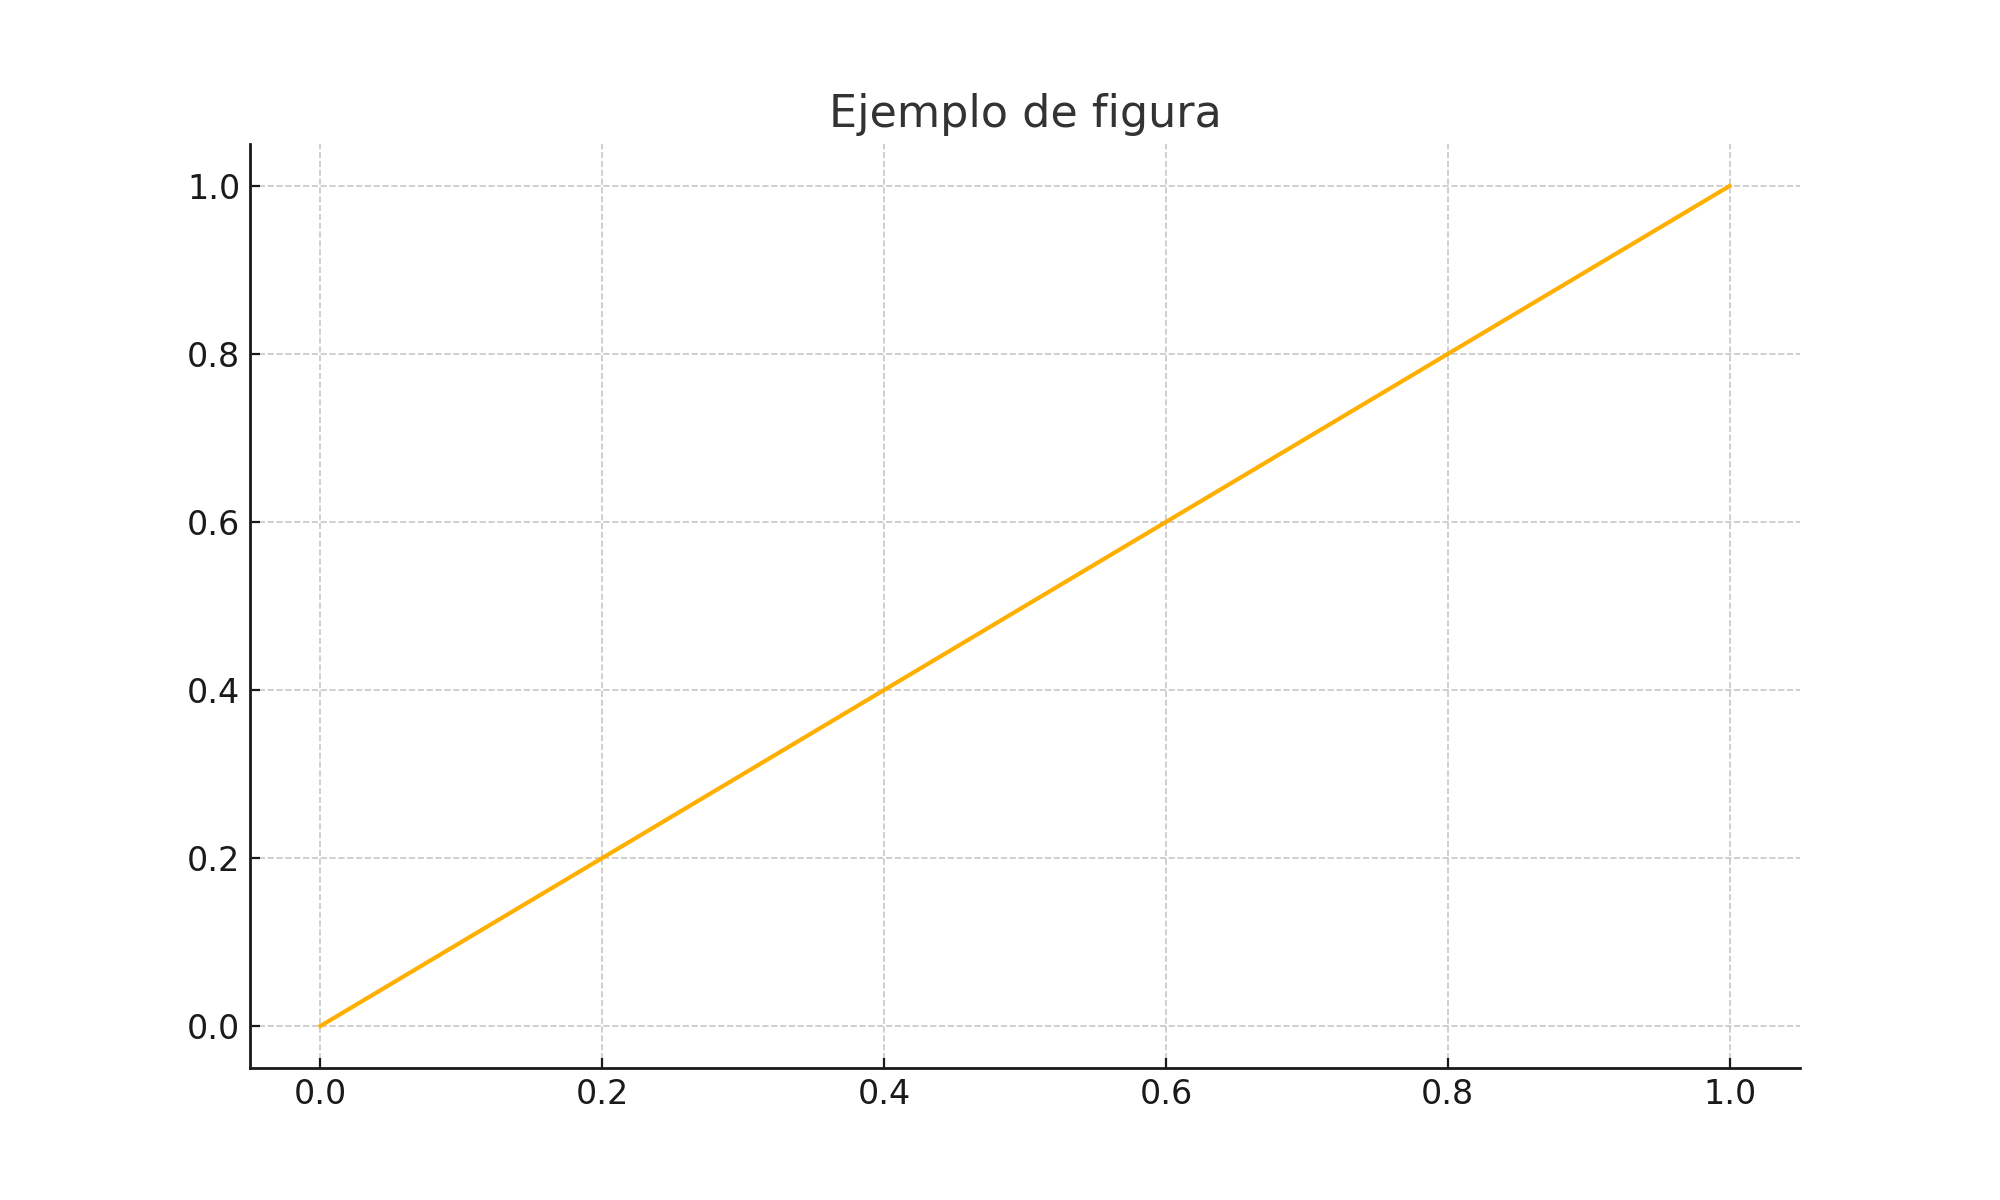
\includegraphics[width=0.7\textwidth]{assets/figura1.png}
\caption{Esquema de fuerzas y su relaci\'on. Fuente: adaptado de Hawking (2010)}
\end{figure}
\subsection*{Tablas}
\begin{table}[H]
\centering
\caption{Participaci\'on de las energías renovables primarias}
\begin{tabular}{|l|l|l|}
\hline
Región & Energías renovables & Biomasa \\
\hline
Latinoam\'erica & 28.9\% & 62.4\% \\
Colombia & 27.7\% & 54.4\% \\
Alemania & 3.8\% & 65.8\% \\
Mundial & 13.1\% & 79.4\% \\
\hline
\end{tabular}
\end{table}

\chapterbreak

\section{Diseño Metodológico}
Describir el enfoque, fases, metodolog\'ia de diagn\'ostico \cite{gonzalezModeloAdministracionProyectos2012} y propuesta de intervenci\'on.

\chapterbreak

% Página horizontal con tabla amplia
\clearpage
\thispagestyle{empty}
\begin{landscape}
\begin{table}[H]
\centering
\caption{Comparativo de tecnologías por país}
\begin{tabular}{|l|c|c|c|c|c|c|}
\hline
País & Solar (MW) & Eólica (MW) & Biomasa (MW) & Hidro (MW) & Geotérmica (MW) & Total Renovables (MW) \\
\hline
Colombia & 100 & 200 & 50 & 1100 & 0 & 1450 \\
Brasil & 500 & 300 & 100 & 2000 & 50 & 2950 \\
Chile & 400 & 450 & 80 & 1200 & 30 & 2160 \\
México & 600 & 700 & 120 & 1800 & 100 & 3320 \\
Perú & 250 & 300 & 60 & 1500 & 20 & 2130 \\
\hline
\end{tabular}
\end{table}
\end{landscape}
\chapterbreak

\section{Diagn\'ostico Organizacional}
\subsection*{Procesamiento estad\'istico de datos}
\subsection*{An\'alisis de resultados}

\chapterbreak

\section{Plan de Intervenci\'on}
Describir la propuesta de mejora/intervenci\'on a implementar.

\chapterbreak

\section{Conclusiones y Recomendaciones}
\subsection*{Conclusiones}
\subsection*{Recomendaciones}

\chapterbreak

\section*{Referencias}
\printbibliography[heading=bibintoc]

\chapterbreak

\appendix
\section*{Anexo A. Nombre del anexo}
Contenido del anexo en esta seccion, puede ser reconocido de forma automatica

\end{document}